
\section{$t=1,2$ The monopolist case}
Consider a similar setting as presented before, with some additional assumptions. The market is a $NxN$ plane. Consumers are uniformally distributed, each consumer that buys from firm $i$ faces an effective price that is influenced by the trading cost to reach firm i as in the following:
\begin{equation}
    P^*(z)=P+tz
\end{equation}
The demand function is the following:
\begin{equation}
q(z)=A \cdot\left[P^*(z)\right]^{-\eta}
\end{equation}
Hence, the quantity demanded decreases with the distance to the firm.
At an initial stage, no firm is in the economy but at time $t_1$ we allow for only one firm to enter. 
We follow a classic formulation of profit:
\begin{equation}
    \Pi=P\cdot Q - mc\cdot Q
\end{equation}
Where $P$ is the price of the monopolist, $Q$ is the total demand she faces and $mc$ is the marginal cost.
The total demand faced by the monopolist is the integral for all the space of the individual space-dependent demand functions:
\begin{equation}
    Q(x_0,y_0)=\int\int_M q(z)=\int\int_M A\cdot\left[P^*(z)\right]^{-\eta}=\int\int_M A \cdot\left[P+tz(x,y;x_0,y_0)\right]^{-\eta}
    \label{eq: max_1}
\end{equation}
Where $M$ is the market area and $x_0, y_0$ is the monopolist location.
$z(x,y;x_0,y_0)$ is the distance between the monopolist and the consumer location. We use the Euclidean Distance, so the equation \ref{eq: max_1} becomes:
\begin{equation}
    Q(x_0,y_0)=\int\int_M A \cdot\left[P+tz(x,y;x_0,y_0)\right]^{-\eta}
    \label{eq: max_2}
\end{equation}
\subsubsection*{The optimal location problem}
Compared to standard microeconomic theory where the monopolist, in a similar setting, only choose $p$ to maximize its profits, in our case the monopolist can choose its location too.
Since the optimal location problem is indipendent from price [this has to be proven probably even if trivial] the monopolist first choose the location and then the best price.
The otpimal location problem is the following:
\begin{equation}
    \max_{x_0,y_0}=Q(x_0,y_0)=\int\int_M q(z)=A \cdot\left[P^*(z)\right]^{-\eta}
\end{equation}
Given the Euclidean distance:
\begin{equation}
z(x,y;x_0,y_0)=\sqrt{(x-x_0)^2+(y-y_0)^2}
\end{equation}
We take the first-order conditions with respect to $x_0$ and $y_0$:
\begin{equation}
\frac{\partial Q}{\partial x_0}=\int\int_M A\cdot(-\eta)\left[P+t\sqrt{(x-x_0)^2+(y-y_0)^2}\right]^{-\eta-1}\cdot\frac{-t(x-x_0)}{\sqrt{(x-x_0)^2+(y-y_0)^2}}=0
\end{equation}
\begin{equation}
\frac{\partial Q}{\partial y_0}=\int\int_M A\cdot(-\eta)\left[P+t\sqrt{(x-x_0)^2+(y-y_0)^2}\right]^{-\eta-1}\cdot\frac{-t(y-y_0)}{\sqrt{(x-x_0)^2+(y-y_0)^2}}=0
\end{equation}
Given the symmetry of the market $M$ (NxN plane), for any point $(x,y)$ there exists a point $(-x,-y)$ such that:
\begin{itemize}
\item The denominator $\sqrt{(x-0)^2+(y-0)^2}=\sqrt{(-x-0)^2+(-y-0)^2}$
\item The terms $(x-0)$ and $(-x-0)$ in the numerator cancel out
\item Similarly, $(y-0)$ and $(-y-0)$ cancel out
\end{itemize}
Therefore, at $(x_0,y_0)=(0,0)$:
\begin{equation}
\frac{\partial Q}{\partial x_0}\bigg|{(0,0)}=0 \quad \text{and} \quad \frac{\partial Q}{\partial y_0}\bigg|{(0,0)}=0
\end{equation}
By locating at the center, the monopolist minimizes the average distance to all consumers, which in turn minimizes the average effective price $P^*(z)$ faced by consumers. At the center, the monopolist ensures symmetric market coverage, where any potential relocation would increase distances to some consumers more than it would decrease distances to others, leading to a net reduction in total demand $Q$.
\subsubsection*{The optimal price problem}
Once the location is chosen, the monopolist set the price that maximize its profits.


Total demand $Q$ is the integral of individual demands over the area:
\begin{equation}
    Q = \iint q(z) \, dA
\end{equation}
Converting to polar coordinates due to radial symmetry:
\begin{equation}
    Q = \int_0^{R} q(z) \cdot 2\pi z \, dz = 2\pi A \int_0^{R} [P + tz]^{-\eta} z \, dz
\end{equation}

Using substitution $u = P + tz$, $du = t \, dz$, $z = \frac{u - P}{t}$:
\begin{equation}
    Q = \frac{2\pi A}{t^2} \int_{u=P}^{u=P + tR} u^{-\eta} (u - P) du
\end{equation}

Expanding the integrand:
\begin{equation}
    u^{-\eta} (u - P) = u^{1-\eta} - Pu^{-\eta}
\end{equation}

Integrating term by term:
\begin{equation}
    Q = \frac{2\pi A}{t^2} \left( \frac{(P + tR)^{2-\eta} - P^{2-\eta}}{2-\eta} - P \cdot \frac{(P + tR)^{1-\eta} - P^{1-\eta}}{1-\eta} \right)
\end{equation}

For large market area ($R \to \infty$) and $\eta > 2$:
\begin{equation}
    Q \approx \frac{2\pi A P^{2-\eta}}{t^2} \left( \frac{1}{\eta-2} + \frac{1}{\eta-1} \right)
\end{equation}

The profit function is:
\begin{equation}
    \Pi = (P-c)Q = K(P-c)P^{2-\eta}
\end{equation}
where $K = \frac{2\pi A}{t^2} \left( \frac{1}{\eta-2} + \frac{1}{\eta-1} \right)$

First-order condition:
\begin{equation}
    \frac{d\Pi}{dP} = K[(P-c)(2-\eta)P^{1-\eta} + P^{2-\eta}] = 0
\end{equation}

Simplifying:
\begin{equation}
    (P-c)(2-\eta) + P = 0
\end{equation}

The optimal price is:
\begin{equation}
    \boxed{P^* = \frac{\eta-2}{\eta-3}c}
\end{equation}
\textbf{Conditions:}
\begin{itemize}
    \item $\eta > 3$ to ensure $P^* > 0$ and profit maximization
    \item Market area must be large enough for the approximation to hold
\end{itemize}
\begin{figure}[H]
    \centering
    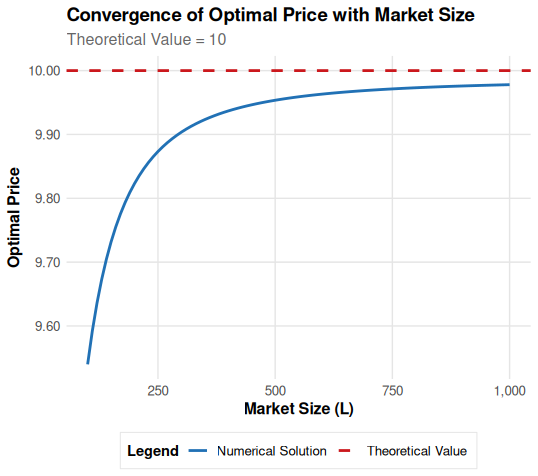
\includegraphics[width=0.7\textwidth]{optimal_price_convergence.png}
    \caption{Convergence of optimal price with market size. The blue solid line shows the numerical solution for different market sizes ($L$), while the red dashed line represents the theoretical value (7.5). Parameter values: demand scale $A=100$, price elasticity $\eta=4$, marginal cost $mc=5$, and transport cost per unit of distance $t=1$. The theoretical price converges to $\frac{\eta-2}{\eta-3}mc = \frac{2}{1}\cdot 5 = 10$ as market size increases, demonstrating the relationship between market size and optimal pricing strategy.}
    \label{fig:price_convergence}
\end{figure}













\section{Introduction}
Hotelling's (1929) spatial competition model, despite its theoretical elegance, has limited empirical applicability due to its restrictive assumptions of linear space, uniform population density, and equidistant firms. The recent advances in computational methods from the spatial economics literature enable us to relax some of these constraints.
We develop a generalized spatial competition framework that maintains Hotelling's core insights while accommodating heterogeneous population distributions and more realistic spatial structures. Our approach progressively relaxes the original model's assumptions, starting from monopolistic location choice and extending to strategic interaction in two-dimensional space. Where closed-form solutions are unavailable, we employ numerical methods.
One of the purpose of this excercise is to show that Hotelling model, and the later circualar case by Salop, are a particular case of this spatial competition framework. The final goal of this research proposal is to create a data friendly model to study the spatial pricing patterns and dynamics.
\section{The general model}

Consider an economy made of a grid with $1,2,...,N$ locations mapped with $x$ and $y$ coordinates in a compact manifold\footnote{This formulation is the same as Allen. Notice that the only 1D closed manifold is the Circle as in the Salop case. While one of the possible 2D compact manifolds is the sphere. See \href{https://en.wikipedia.org/wiki/Closed_manifold}{here}} $S$ in $\mathbb{R}^2$. In this economy lives $M$ immobile consumers, where at any location $s \in S$ the density of consumers is represented by a density function $\rho(s) \geq 0$. The total number of consumers in the economy is hence:

\begin{equation}
\int_S \rho(s)ds = M
\end{equation}

The functions $\rho: S \rightarrow \mathbb{R}_+$ and $d: S \times S \rightarrow [0,1]$ comprise the geography of the market, where $d(s,s')$ represents the fraction of value lost when transporting goods between locations $s$ and $s'$. I assume that (a) $\rho$ is continuous and bounded and (b) $d$ is a distance metric on $S$; apart from these restrictions, the geography is otherwise flexible.

\subsection{Firms and Consumers}

A fixed number of firms $i \in \{1,...,N\}$ compete in this market. Each firm charges a price $p_i$ for its homogeneous product and incurs a fixed cost $F$ for operation. Production cost $c$ is equal for all firms. A consumer located at $s \in S$ who buys from firm $i$ located at $x_i$ faces an effective price that incorporates both the mill price and transportation costs:

\begin{equation}
P^*_i(s) = p_i(1 + d(s,x_i))
\end{equation}

Consumers have constant elasticity demand:
\begin{equation}
q(s) = A \cdot [P^*_i(s)]^{-\eta}
\end{equation}

As mentioned by Barro 2024, this demand structure arises from utility maximization where consumers maximize:
\begin{equation}
U_i(s) = \frac{\eta}{\eta-1}q(s)^{(\eta-1)/\eta} + \hat{q}
\end{equation}
subject to the budget constraint:
\begin{equation}
Y = P^*_i(s)q(s) + \hat{q}
\end{equation}
where $\hat{q}$ is a numeraire good.
\subsection{Market Areas and Strategic Competition}

For any given configuration of firm locations $\{x_i\}_{i=1}^N$ and prices $\{p_i\}_{i=1}^N$, each firm $i$ commands a market area $V_i \subseteq S$, which consists of all locations where consumers find it optimal to purchase from firm $i$. These market areas are the outcome of consumers' optimal choices, reflecting both spatial preferences and the strategic interaction between firms.

Formally, the market area for firm $i$ is defined as the set of locations $s \in S$ where the price at firm $i$, adjusted for distance, is no higher than the price at any competitor, also adjusted for the corresponding distance. This can be expressed as:

\[
V_i(p,x) = \{ s \in S \mid p_i(1 + d(s,x_i)) \leq p_j(1 + d(s,x_j)) \text{ for all } j \neq i \},
\]

where $d(s, x_i)$ represents the distance between location $s$ and the location of firm $i$, and $p_i$ is the price charged by firm $i$.

The structure of these market areas depends on several factors, both spatial and strategic. On the one hand, firms face a fundamental tradeoff when setting prices. Lowering prices generally expands the firm's market area, since $\frac{\partial |V_i|}{\partial p_i} < 0$, but this also reduces the per-unit profit, with $\frac{\partial (p_i - c)}{\partial p_i} > 0$, where $c$ is the firm's marginal cost. On the other hand, the precise shape of market areas is influenced by various elements: the geographic distance between consumers and firms, the relative prices across firms, consumer density, and the locations of competing firms.

In the special case where all firms charge the same price ($p_i = p_j$ for all $i,j$), the market areas simplify to Voronoi regions, where each firm serves the closest consumers. This configuration is illustrated in Figure \ref{fig:voronoi_regions} and can be expressed as:

\[
V_i = \{ s \in S \mid d(s,x_i) \leq d(s,x_j) \text{ for all } j \neq i \}.
\]

When prices are different across firms, however, market areas deviate from Voronoi shapes. The boundaries between the market areas of any two firms are determined by hyperbolic curves, which satisfy the following condition:

\[
d(s,x_j) - d(s,x_i) = \frac{p_i - p_j}{t},
\]

where $t$ is a parameter related to the sensitivity of consumers to price differences.

The size and shape of these market areas have direct implications for firm profits, affecting them through two primary channels. First, the market size effect, which is the impact of changes in market area on profits, can be expressed as:

\[
\frac{\partial \pi_i}{\partial |V_i|} = (p_i - c)\int_{\partial V_i} \rho(s) q(s) \, ds > 0,
\]

where $\rho(s)$ represents consumer density at location $s$, and $q(s)$ is the quantity demanded at $s$. This term captures how an increase in the market area increases firm profits through greater market size.

Second, the price-cost margin effect reflects the sensitivity of profits to changes in the firm's price. It can be written as:

\[
\frac{\partial \pi_i}{\partial p_i} = D_i + (p_i - c)\frac{\partial D_i}{\partial p_i},
\]

where $D_i$ denotes the demand for firm $i$'s product, and $\frac{\partial D_i}{\partial p_i}$ captures how demand responds to price changes. Both these effects highlight the interplay between spatial considerations and strategic pricing in shaping the competitive landscape.


\subsection{Dynamic Competition}
This section examines dynamic competition in a two-dimensional spatial market, where firms make both price and location decisions. The problem is complex due to the interplay between pricing and location choices, which leads to non-concavities in the profit functions and may give rise to multiple local optima.

To address the challenges of simultaneous maximization, we adopt a \textit{dynamic approach} similarly to Allen. Time \( t \in \{0,1,...\} \) is discrete, with firms alternating between optimizing prices and locations:

\begin{itemize}
    \item \textbf{For odd \( t \)}, firms simultaneously choose prices, holding locations fixed:
    \[
        p_{it} = \arg\max_{p_i} \pi_i(p_i, p_{-i,t}, x_{t-1}).
    \]
    \item \textbf{For even \( t \)}, firms simultaneously choose locations, given the previous period's prices:
    \[
        x_{it} = \arg\max_{x_i} \pi_i(p_{t-1}, x_i, x_{-i,t}).
    \]
\end{itemize}
This alternating structure ensures that each optimization problem is well-behaved, with clear first-order conditions and existence results. Moreover, this framework guarantees that the equilibrium path is unique and converges to a steady state.

A \textit{dynamic equilibrium} for geography \( \{\rho,d\} \) and initial locations \( \{x_{i0}\}_{i \in N} \) is defined as the set of prices and locations \( \{p_{it}, x_{it}\}_{i \in N, t \in T} \) such that:

\begin{itemize}
    \item For odd \( t \) (price setting), prices satisfy:
    \[
        p_{it} = \arg\max_{p_i} (p_i - c) \int_{V_i(p_i, p_{-i,t}, x_{t-1})} \rho(s) A [p_i(1 + d(s, x_{i,t-1}))]^{-\eta} \, ds - F
    \]
    \item For even \( t \) (location setting), locations satisfy:
    \[
        x_{it} = \arg\max_{x_i} (p_{i,t-1} - c) \int_{V_i(p_{t-1}, x_i, x_{-i,t})} \rho(s) A [p_{i,t-1}(1 + d(s, x_i))]^{-\eta} \, ds - F.
    \]
\end{itemize}

A \textit{steady state} is a set of prices and locations \( \{p^*_i, x^*_i\}_{i \in N} \) that satisfies both conditions simultaneously.

\begin{proposition}[Price Equilibrium]  
For any given set of locations \( x \), a unique price equilibrium exists if:
\begin{enumerate}
    \item The transportation cost function \( d \) is continuous.
    \item The demand elasticity \( \eta > 1 \).
    \item The consumer density \( \rho \) is bounded.
\end{enumerate}
\end{proposition}

\begin{proof}
These conditions ensure the existence and uniqueness of equilibrium through standard mechanisms:
\begin{itemize}
    \item Continuity of \( d \) ensures that the demand functions are continuous in price, preventing any discontinuities in market areas as prices change. This smoothness is crucial for the existence of a price equilibrium.
    \item Demand elasticity \( \eta > 1 \) ensures that demand is sufficiently elastic, which makes each firm's profit function strictly concave in its own price. If \( \eta \leq 1 \), the profit function becomes unbounded, and firms would have an incentive to raise prices indefinitely, eliminating equilibrium.
    \item Boundedness of \( \rho \) ensures that the consumer mass at any location is finite, preventing the emergence of degenerate equilibria where firms focus solely on an infinitely large consumer mass at a single location.
\end{itemize}

Together, these conditions guarantee that each firm's profit function is continuous, strictly concave, and has a well-defined global maximum, ensuring the existence of a pure-strategy Nash equilibrium in prices by standard results from game theory.

Uniqueness follows from the strict concavity of each firm's profit function and the strategic complementarity of prices, meaning that when one firm raises its price, the other firms are also incentivized to increase their prices. This ensures that the best-response functions intersect exactly once, guaranteeing a unique equilibrium price for each firm.
\end{proof}

\begin{proposition}[Price Competition Properties]  
The price equilibrium has the following properties:
\begin{enumerate}
    \item Prices are \textit{strategic complements}: \( \frac{\partial p^*_i}{\partial p_j} > 0 \).
    \item Markups \textit{decrease with transportation costs}: \( \frac{\partial (p^*_i - c)}{\partial t} < 0 \).
    \item Markups \textit{decrease with demand elasticity}: \( \frac{\partial (p^*_i - c)}{\partial \eta} < 0 \).
    \item Markups \textit{increase with distance to competitors}: \( \frac{\partial (p^*_i - c)}{\partial d(x_i, x_j)} > 0 \).
\end{enumerate}
\end{proposition}

\subsection{Location Choice}

Given the price equilibrium \( p^*(x) \), we now characterize the location equilibrium.

\begin{proposition}[Location Equilibrium]
For any given configuration of equilibrium prices $p^*$, a location equilibrium exists if:
\begin{enumerate}
    \item The space $S$ is convex
    \item The transportation cost function $d$ is convex in firm locations
\end{enumerate}
\end{proposition}

\begin{proof}
Given equilibrium prices $p^*$, a firm's profit at location $x_i$ can be written as:
\[
\pi_i(x_i, x_{-i}) = \int_{V_i(x_i, x_{-i})} \rho(s)(p^*_i - c)(1 - d(s,x_i)) \, ds
\]
where $V_i(x_i, x_{-i})$ is the market area of firm $i$ defined by:
\[
V_i = \{s \in S: p^*_i(1 + d(s,x_i)) \leq p^*_j(1 + d(s,x_j)) \text{ for all } j \neq i\}
\]

The proof proceeds in three steps:

1) First, note that given convexity of $S$, the strategy space for each firm is compact and convex.

2) The profit function is continuous in $x_i$ because:
   \begin{itemize}
      \item $d(s,x_i)$ is continuous by assumption
      \item Changes in market area boundaries have measure zero due to convexity of $d$
      \item Integration over $V_i$ is continuous by the dominated convergence theorem
   \end{itemize}

3) The profit function is quasi-concave in $x_i$ because:
   \begin{itemize}
      \item Convexity of $d$ implies that for any $\lambda \in [0,1]$ and locations $x, y$:
      \[
      d(s,\lambda x + (1-\lambda)y) \leq \lambda d(s,x) + (1-\lambda)d(s,y)
      \]
      \item This ensures that any profitable deviation must be local rather than global
      \item The market area $V_i$ is continuous in $x_i$ due to convexity of $d$
   \end{itemize}

Therefore, by Kakutani's fixed point theorem, a pure strategy Nash equilibrium in locations exists.
\end{proof}

\begin{remark}
The convexity conditions serve two crucial purposes:
\begin{itemize}
    \item They ensure continuity of payoffs by ruling out discontinuous changes in market areas
    \item They create a tradeoff between market size and price competition that makes the profit function well-behaved
\end{itemize}
\end{remark}

\begin{proposition}[Location Choice Properties]  
In equilibrium, firms exhibit the following location choice patterns:
\begin{enumerate}
    \item Firms \textit{locate further apart} as transportation costs increase.
    \item Firms \textit{cluster more} in areas of high consumer density.
    \item Location choices become \textit{more dispersed} as demand becomes more elastic.
\end{enumerate}
\end{proposition}

\subsection{Dynamic Properties}

We now examine the properties of the dynamic equilibrium.

\begin{proposition}[Convergence]  
Under the conditions for the existence of price and location equilibria, the dynamic equilibrium converges to a steady state.  
\end{proposition}

\begin{proof}
This follows from standard results in dynamic game theory and the fact that each alternating optimization step leads to a unique equilibrium in each subgame. The system converges to a steady state because each stage (price and location choice) has well-behaved equilibria that guide the system toward a unique limiting configuration.
\end{proof}

\begin{proposition}[Steady State Multiplicity]  
While multiple steady states may exist, the dynamic path and limiting steady state are unique given initial conditions \( \{x_{i0}\}_{i \in N} \).
\end{proposition}

\begin{proof}
The uniqueness of the limiting steady state is ensured by the alternating structure of the game and the properties of the optimization problems at each stage. This ensures that, despite the potential for multiple steady states in static models, the dynamic process leads to a single steady state.
\end{proof}

\subsection{Efficiency}

\begin{proposition}[Efficiency]  
Any steady state is locally efficient in that:
\begin{enumerate}
    \item Price deviations cannot improve aggregate consumer surplus net of costs.
    \item Location deviations cannot improve aggregate consumer surplus net of costs.
\end{enumerate}
\end{proposition}

\begin{proof}
This follows from standard efficiency results in spatial models with firm competition. Any deviation in price or location would reduce the total surplus, given that firms are already maximizing their profits in response to each other.
\end{proof}







This alternating structure has several advantages in terms of analytical traceability. Each stage has well-behaved optimization with clear first-order conditions and existence and uniqueness results.

Moreover, this structure allows us to establish three key results:

\begin{proposition}[Dynamic Properties]
Under the alternating structure:
\begin{enumerate}
    \item A dynamic equilibrium exists
    \item Given initial conditions, the equilibrium path is unique
    \item The equilibrium converges to a steady state
\end{enumerate}
\end{proposition}

The intuition is that price competition, holding locations fixed, has a unique equilibrium. Given these prices, location choices also have a unique equilibrium. The alternation between these well-behaved stages drives the system toward a stable configuration.

This approach builds on computational geometry literature on Lloyd's algorithm and Centroidal Voronoi Tessellations (CVT), but extends it to account for:
\begin{itemize}
    \item Price competition
    \item Strategic interaction
    \item Variable consumer density
    \item General transportation costs
\end{itemize}

The framework thus provides a tractable way to analyze how market structure evolves through the interaction of price and location decisions while maintaining both theoretical rigor and economic insight.


\section{The general model}
Consider an economy comprised of a compact manifold $S$ in $\mathbb{R}^2$. Each point $s \in S$ is endowed with a density of consumers $\rho(s) \geq 0$. We make two initial assumptions about the geography:

Consider an economy made of a grid with 1, 2, ..., N locations mapped with $x$ and $y$ coordinates.
In this economy lives M immobile consumers and at any location L(x,y) the density of consumers is represented by a density function $\rho(x,y)$.
The total number of consumers in the economy is hence:
\begin{equation}
\int_0^1 \int_0^1 \rho(x, y) d x d y=M
\end{equation}
Each firm $i$ charges a price $p_i$ for its product which is homogeneous and among firms and incurs a fixed cost F for operation. Production cost is equal for all the firms. A firm can decide to enter the market incurring a one-time entry cost E.
Consumers derive utility from purchasing the product and the consumer located at $(x,y)$ who buys from firm $i$ located at $(x_i,y_i)$. The price is influenced by transportation cost.
\begin{equation}
P^*_i(x,y)=p_i+t \cdot z
\end{equation}
Where $z$ is the Euclidean Distance from firm $i$ and consumer located in $x,y$. $t$ is the transportation cost.

The demand to a firm of a consumer with distance $z$ depends on the effective price faced and is:
\begin{equation}
q(z)=A \cdot\left[P^*(z)\right]^{-\eta}
\end{equation}
This is a constant elasticity demand function which depend on the effective price, namely price with transport cost. This is implied from  Anderson and de Palma (2000) and Gu and Wenzel (2009) by a utility function of the form:
\begin{equation}
U_i(z)=\frac{\eta}{\eta-1} q(z)^{(\eta-1) / \eta}+\hat{q}
\end{equation}
where $\hat{q}$ is the quantity of a numeraire good and gross income is:
\begin{equation}
Y=P^*(z) \cdot q(z)+\hat{q}.
\end{equation}


We draw on tools from computational geometry and the theory of shape optimization to draw the boundaries where a consumer is indifferent between firm $i$ and $j$.
Firms compete for consumers based on location and price. Consumers will choose the firm that maximizes their utility. This competition defines strict preference regions around each firm, which are geometric regions where each consumer is closest to a particular firm.
The following condition defines the indifference boundary:
\begin{equation}
P^*_i(x, y)=P^*_j(x, y)
\end{equation}
Simplifying we get:
\begin{equation}
    p_i+tz_i=p_j+tz_j
\end{equation}
\begin{equation}
    \frac{p_i-p_j}{t}=z_j-z_i
    \label{eq:voronoi}
\end{equation}
This hyperbolic boundary separates the regions of strict preference areas of firms $i$ and $j$.
The strict preference region for firm $i$ can be described as the region where all the customers in it face lower price from firm $i$ than from any other firm. This region is defined as:
\begin{equation}
V_i(x, y)=\left\{(x, y) \mid P_i(x, y)<P_j(x, y) \text { for all } j \neq i\right\}
\end{equation}
We then define the total demand $D_i$ for firm $i$ as the integral of the consumer density function $\rho(x,y)$ over the firm's strict preference region $V_i$ which contains all consumers closest to that firm:
\begin{equation}
D_i=\int_{V_i} \rho(x, y) \cdot q(z) d x d y
\label{eq:demand}
\end{equation}
Which can be rewritten as:
\begin{equation}
D_i=\int_{V_i} \rho(x, y) \cdot A \cdot\left[p_i+t \cdot \sqrt{\left(x-x_i\right)^2+\left(y-y_i\right)^2}\right]^{-\eta} d x d y
\end{equation}
This gives the total demand that firm $i$ captures based on its position, the positions of the other firms and its pricing.
Each firm seeks to maximise its profit by setting the optimal price $p_i$ and choosing a location that maximizes its market share.
The profit $\pi_i$ of firm $i$ is given by:
\begin{equation}
    \pi_i=p_i\cdot D_i- c\cdot D_i -F
\end{equation}
Where:
\begin{itemize}
    \item $p_i$ is the price charged by firm $i$.
    \item $D_i$ is the demand captured by firm $i$.
    \item $c$ is the constant marginal cost of producing the good.
    \item F is the fixed cost of the firm.
\end{itemize}
To find the profit-maximising price we take the derivative of profit function with respect to price:
\begin{equation}
\frac{\partial \pi_i}{\partial p_i}=D_i+p_i \cdot \frac{\partial D_i}{\partial p_i}-c \cdot \frac{\partial D_i}{\partial p_i}=0
\end{equation}
Price determines the strict preference region and it enters in the demand as in function \ref{eq:demand} and \ref{eq:voronoi}.
Simplifying, we obtain the markup condition:
\begin{equation}
p_i-c=-\frac{D_i}{\frac{\partial D_i}{\partial p_i}}
\end{equation}
Thus, the markup $p_i-c$ depends on the demand elasticity 
$\eta$ and how demand changes with respect to the price (as reflected in the first-order condition). The higher the elasticity, the smaller the markup.
\subsubsection*{Firm entry and exit decision}
At each iteration a firms out of the market can decide to enter and incumbent can decide to leave.
A new firm entry the market if its expected profit is positive after paying the entry cost E. The firm evaluate the potential demand it can capture based on the consumer density and the locations of existing competitors. Hence, firm i enters the market if:
\begin{equation}
\pi_i=p_i \cdot D_i-F-E>0
\end{equation}.
The new firms must also decide where to enter the market and it chooses an optimal location $x_i^*,y_i^*$ such that its profit is maximised considering both the existing firms and the consumer density distribution.
\begin{equation}
\left(x_i^*, y_i^*, p_i\right)=\arg \max _{(x, y, p_i)}\left(p_i \cdot D_i(x, y)-F-E\right)
\end{equation}
New firms enter sequentially, each choosing an optimal location and setting a price to maximize profits. The process continues until no additional firm can profitably enter the market. The entry process stops when the following condition holds for every potential entrant:
$$
\pi_i<0 \text { for all remaining potential entrants }
$$
Each period firms fail and exit the market when the following condition is true:
\begin{equation}
\pi_i=p_i \cdot D_i-F-E<0
\end{equation}.
\section{Some thoughts on equilibrium}
Equilibrium existence and uniqueness has to be proven.
In equilibrium, firms are distributed across the market in such a way that no firm can improve its position or profits by relocating or changing its price.
Each firm captures a portion of the market and their prices are adjusted to balance competition.
Some price and location inefficiencies are allowed for the entry costs. 
\begin{figure}
    \centering
    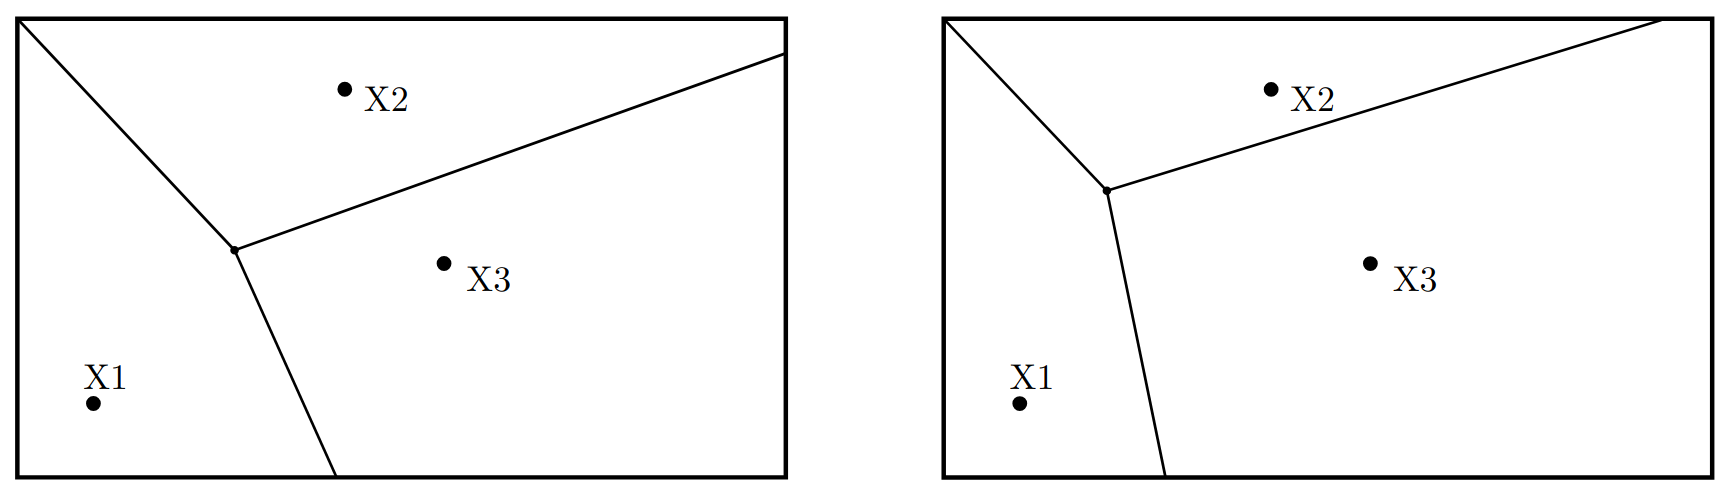
\includegraphics[width=1\linewidth]{image.png}
    \caption{Voronoi regions}
    \label{fig:voronoi_regions}
\end{figure}




\section{Duopoly (It has to be proven for small R)}
We now consider the case of two firms (\( i = 1, 2 \)) located at positions \( (x_i, y_i) \) in a two-dimensional plane. Consumers are uniformly distributed over the plane and incur transportation costs when purchasing from firms. Each firm sets its price \( P_i \) to maximize its profit, taking into account the presence of the other firm.

Again, for a consumer located at \( (x, y) \), the effective price of purchasing from firm \( i \) is:

\[
P_i^{\text{eff}}(x, y) = P_i + t \cdot d_i(x, y)
\]

where \( P_i \) is the price set by firm \( i \),
\( t \) is the transportation cost per unit distance, and \( d_i(x, y) \) is the Euclidean distance between the consumer and firm \( i \).

Consumers choose the firm offering the lowest effective price. That is, a consumer at \( (x, y) \) will choose firm 1 if:

\[
P_1^{\text{eff}}(x, y) \leq P_2^{\text{eff}}(x, y)
\]

The market area for firm 1 is the set of all points \( (x, y) \) satisfying the above inequality. The boundary between the market areas of the two firms is defined by the set of points where:

\[
P_1^{\text{eff}}(x, y) = P_2^{\text{eff}}(x, y)
\]

Substituting the expression for effective prices:

\[
P_1 + t \cdot d_1(x, y) = P_2 + t \cdot d_2(x, y)
\]

Rewriting:

\[
t \left[ d_2(x, y) - d_1(x, y) \right] = P_1 - P_2
\]

Let \( \Delta P = P_1 - P_2 \). The boundary is then given by:

\[
d_2(x, y) - d_1(x, y) = \frac{\Delta P}{t}
\]

This equation represents a hyperbola in the plane separating the market areas of the two firms.

\subsection{Demand for Firm 1}

The demand faced by firm 1 is:

\[
Q_1 = \int_{\text{Region}_1} A \left[ P_1^{\text{eff}}(x, y) \right]^{-\eta} \, dx \, dy
\]

Similarly for firm 2:

\[
Q_2 = \int_{\text{Region}_2} A \left[ P_2^{\text{eff}}(x, y) \right]^{-\eta} \, dx \, dy
\]

\subsection{Simplifying Assumptions}

To obtain analytical tractability, we make the following assumptions:
\begin{itemize}
    \item Symmetric Locations: Firms are symmetrically located along the \( x \)-axis at \( (-d, 0) \) and \( (d, 0) \).
    \item Equal Pricing: Firms charge the same price, \( P_1 = P_2 = P \).
    \item Infinite Market: The market extends infinitely in all directions.
    \item Uniform Consumer Distribution: Consumers are uniformly distributed over the plane.
\end{itemize}

Under these assumptions, the boundary between the market areas becomes the perpendicular bisector of the line segment joining the two firms, which is the \( y \)-axis (\( x = 0 \)).
For firm 1, the effective price is:

\[
P_1^{\text{eff}}(x, y) = P + t \cdot \sqrt{(x + d)^2 + y^2}
\]

Consumers to the left of \( x = 0 \) choose firm 1. Therefore, the demand for firm 1 is:

\[
Q_1 = \int_{x = -\infty}^{x = 0} \int_{y = -\infty}^{y = \infty} A \left[ P_1^{\text{eff}}(x, y) \right]^{-\eta} \, dy \, dx
\]

Similarly for firm 2:

\[
Q_2 = \int_{x = 0}^{x = \infty} \int_{y = -\infty}^{y = \infty} A \left[ P_2^{\text{eff}}(x, y) \right]^{-\eta} \, dy \, dx
\]

Since the firms are symmetrically located and charge the same price, \( Q_1 = Q_2 \).

Now let's calculate \( Q_1 \):

\[
Q_1 = A \int_{x = -\infty}^{0} \int_{y = -\infty}^{\infty} \left[ P + t \cdot \sqrt{(x + d)^2 + y^2} \right]^{-\eta} \, dy \, dx
\]

We can switch to polar coordinates centered at \( (-d, 0) \):

Let:

\[
\begin{cases}
x + d = r \cos \theta \\
y = r \sin \theta
\end{cases}
\]

where $r$ is the Jacobian determinant. 
The limits of integration for \( r \) are from \( 0 \) to \( \infty \), and for \( \theta \) from \( \theta = \pi \) to \( \theta = 2\pi \) (since \( x \leq 0 \)).

Thus, the demand becomes:

\[
Q_1 = A \int_{\theta = \pi}^{2\pi} \int_{r = 0}^{\infty} \left[ P + t \cdot r \right]^{-\eta} r \, dr \, d\theta
\]

Integrate over \( \theta \):

\[
Q_1 = A \left( \int_{\theta = \pi}^{2\pi} d\theta \right) \left( \int_{r = 0}^{\infty} \left[ P + t \cdot r \right]^{-\eta} r \, dr \right)
\]

Since \( \int_{\theta = \pi}^{2\pi} d\theta = \pi \), we have:

\[
Q_1 = A \pi \int_{r = 0}^{\infty} \left[ P + t \cdot r \right]^{-\eta} r \, dr
\]

Let \( u = P + t \cdot r \), then \( du = t \, dr \), so \( dr = \frac{du}{t} \). When \( r = 0 \), \( u = P \); as \( r \to \infty \), \( u \to \infty \).

Also, \( r = \frac{u - P}{t} \).

Substitute into the integral:

\[
Q_1 = A \pi \int_{u = P}^{\infty} u^{-\eta} \left( \frac{u - P}{t} \right) \left( \frac{du}{t} \right)
\]

Simplify:

\[
Q_1 = \frac{A \pi}{t^2} \int_{u = P}^{\infty} u^{-\eta} (u - P) \, du
\]

\subsection{Evaluating the Integral}

Let \( I = \int_{u = P}^{\infty} u^{-\eta} (u - P) \, du \)

Let \( v = u - P \), then \( u = v + P \), when \( u = P \), \( v = 0 \), as \( u \to \infty \), \( v \to \infty \).

Substitute:

\[
I = \int_{v = 0}^{\infty} (v + P)^{-\eta} v \, dv
\]

This integral can be evaluated using standard integral formulas.

Let’s expand \( (v + P)^{-\eta} \) in terms of \( v \):

But to proceed, we'll consider that \( P \) is constant with respect to \( v \). The integral becomes:

\[
I = \int_{v = 0}^{\infty} (v + P)^{-\eta} v \, dv
\]

This integral can be evaluated by making a substitution or using the Beta function.

However, for \( \eta > 2 \), the integral converges, and we can write:

\[
I = \frac{P^{2 - \eta}}{(\eta - 2)(\eta - 1)}
\]

Therefore, the demand for firm 1 is:

\[
Q_1 = \frac{A \pi P^{2 - \eta}}{t^2 (\eta - 2)(\eta - 1)}
\]

Similarly for firm 2.

\subsection{Profit Maximization}

Each firm seeks to maximize its profit:

\[
\Pi_i = (P - mc) Q_i
\]

Substituting the expression for \( Q_i \):

\[
\Pi_i = \frac{A \pi (P - mc) P^{2 - \eta}}{t^2 (\eta - 2)(\eta - 1)}
\]

To find the optimal price \( P^* \), we take the derivative of \( \Pi_i \) with respect to \( P \) and set it to zero:

\[
\frac{d\Pi_i}{dP} = 0
\]

Compute the derivative:

\[
\frac{d\Pi_i}{dP} = \frac{A \pi}{t^2 (\eta - 2)(\eta - 1)} \left[ (P - mc)(2 - \eta) P^{1 - \eta} + P^{2 - \eta} \right]
\]

Set the derivative to zero:

\[
(P - mc)(2 - \eta) P^{1 - \eta} + P^{2 - \eta} = 0
\]

Divide both sides by \( P^{1 - \eta} \):

\[
(P - mc)(2 - \eta) + P = 0
\]

Simplify:

\[
(2 - \eta)(P - mc) + P = 0
\]

Rewriting:

\[
(2 - \eta) P + (\eta - 2) mc + P = 0
\]

Combine like terms:

\[
(3 - \eta) P + (\eta - 2) mc = 0
\]

Solve for \( P \):

\[
(3 - \eta) P = (2 - \eta) mc
\]

Multiply both sides by \( -1 \):

\[
(\eta - 3) P = (\eta - 2) mc
\]

Therefore, the optimal price is:

\[
P^* = \frac{\eta - 2}{\eta - 3} mc
\]

**Note**: This solution is valid only if \( \eta > 3 \), ensuring \( P^* > 0 \).

\subsection{Summary}

- **Optimal Price**:

  \[
  P^* = \frac{\eta - 2}{\eta - 3} mc
  \]

- **Demand for Each Firm**:

  \[
  Q_i = \frac{A \pi P^{2 - \eta}}{t^2 (\eta - 2)(\eta - 1)}
  \]

- **Profit for Each Firm**:

  \[
  \Pi_i = \frac{A \pi (P - mc) P^{2 - \eta}}{t^2 (\eta - 2)(\eta - 1)}
  \]

---

This completes the analytical derivation for the duopoly case, providing expressions for the optimal price, demand, and profit for each firm in a symmetric duopoly setting on a two-dimensional plane.



\appendix
\section*{Mathematical Appendix}

\subsection*{Analytical Derivation of the Equilibrium Price}

Let the profit of firm \( i \) at time \( t \) be denoted by \( \pi_i(p_i, x_i, p_{-i}, x_{-i}) \), which depends on the firm's own price \( p_i \), its location \( x_i \), the prices \( p_{-i} \) of the other firms, and their locations \( x_{-i} \). The profit function is given by:

\[
\pi_i(p_i, x_i, p_{-i}, x_{-i}) = (p_i - c) \int_{V_i(p_i, x_i, p_{-i}, x_{-i})} \rho(s) A \left[ p_i (1 + d(s, x_i)) \right]^{-\eta} \, ds - F,
\]

where:

\begin{itemize}
    \item \( (p_i - c) \) is the price-cost margin,
    \item \( \int_{V_i} \rho(s) A \left[ p_i (1 + d(s, x_i)) \right]^{-\eta} \, ds \) is the total revenue from customers in firm \( i \)'s market area \( V_i \),
    \item \( F \) is the fixed cost of the firm,
    \item \( \rho(s) \) is the consumer density at location \( s \),
    \item \( A \) is a scaling constant, and
    \item \( \eta \) is the price elasticity of demand.
\end{itemize}

To find the equilibrium price, we take the derivative of the profit function with respect to \( p_i \) and set it equal to zero. This yields the first-order condition for price maximization:

\[
\frac{\partial \pi_i}{\partial p_i} = 0.
\]

First, we differentiate the two components of the profit function:

1. **Differentiating the price-cost margin**:

\[
\frac{\partial}{\partial p_i} (p_i - c) = 1.
\]

2. **Differentiating the demand integral**:

To differentiate the integral, we apply the Leibniz rule for differentiation under the integral sign:

\[
\frac{\partial}{\partial p_i} \int_{V_i} \rho(s) A \left[ p_i (1 + d(s, x_i)) \right]^{-\eta} \, ds = \int_{\partial V_i} \rho(s) A \left( -\eta \left[ p_i (1 + d(s, x_i)) \right]^{-\eta-1} (1 + d(s, x_i)) \right) \, ds,
\]

where \( \partial V_i \) denotes the boundary of the market area \( V_i \), as the change in the market area depends on the price.

Thus, the first-order condition becomes:

\[
\frac{\partial \pi_i}{\partial p_i} = 1 - (p_i - c) \eta \int_{\partial V_i} \rho(s) A \left[ p_i (1 + d(s, x_i)) \right]^{-\eta-1} (1 + d(s, x_i)) \, ds = 0.
\]

Simplifying, we have:

\[
1 - (p_i - c) \eta \int_{\partial V_i} \rho(s) A \left[ p_i (1 + d(s, x_i)) \right]^{-\eta-1} (1 + d(s, x_i)) \, ds = 0.
\]

Rearranging:

\[
(p_i - c) = \frac{1}{\eta \int_{\partial V_i} \rho(s) A \left[ p_i (1 + d(s, x_i)) \right]^{-\eta-1} (1 + d(s, x_i)) \, ds}.
\]

At this point, we observe that the equilibrium price \( p_i^* \) can be implicitly defined by this equation.

\subsection*{Equilibrium Price Expression}

Under the assumption that the market area \( V_i \) is fixed for a given price, the equilibrium price can be approximated by the following expression:

\[
p_i^* - c = \frac{D_i}{\eta D_i + \int_{\partial V_i} \rho(s) q(s) \|\nabla d(s, x_i)\| \, ds},
\]

where:

\begin{itemize}
    \item \( D_i \) is the total demand in firm \( i \)'s market area,
    \item \( q(s) \) is the demand at location \( s \),
    \item \( \|\nabla d(s, x_i)\| \) is the gradient of the transportation cost function \( d(s, x_i) \) with respect to location \( x_i \), and
    \item The integral represents the change in the market area boundary with respect to price.
\end{itemize}

This equation expresses the equilibrium price \( p_i^* \) in terms of the demand, transportation costs, and consumer density, reflecting the strategic interactions between firms in the spatial market.

\subsection*{Uniqueness of the Equilibrium}

The uniqueness of the equilibrium price follows from the concavity of the profit function, which is guaranteed under the following conditions:

\begin{itemize}
    \item The transportation cost function \( d \) is continuous,
    \item The demand elasticity \( \eta > 1 \), and
    \item The consumer density \( \rho \) is bounded.
\end{itemize}

These conditions ensure that the profit function is strictly concave in \( p_i \), implying that there is a unique solution for the equilibrium price \( p_i^* \).

\subsection*{Conclusion}

The equilibrium price is determined by the first-order condition for profit maximization, which balances the firm's markup over cost with the effects of demand elasticity, transportation costs, and consumer density. The equilibrium is unique due to the strict concavity of the profit function under the stated assumptions. This equilibrium price characterizes the spatial competition between firms in the model.
\section{Introduction nuovo. Valutare se buono}

Hotelling's (1929) spatial competition model, despite its theoretical elegance, has limited empirical applicability due to its restrictive assumptions of linear space, uniform population density, and equidistant firms. Recent advances in computational methods in spatial economics enable us to relax some of these constraints.

We develop a generalized spatial competition framework that maintains Hotelling's core insights while accommodating heterogeneous population distributions and more realistic spatial structures. Our approach progressively relaxes the original model's assumptions, starting from monopolistic location choice and extending to strategic interaction in two-dimensional space. Where closed-form solutions are unavailable, we employ numerical methods.

One purpose of this exercise is to show that Hotelling's model and the later circular case by Salop are particular instances of this spatial competition framework. The final goal of this research is to create a data-friendly model to study spatial pricing patterns and dynamics.

\section{The General Model}

Consider an economy represented by a compact, convex subset \( S \subset \mathbb{R}^2 \), which denotes the spatial market. Consumers are distributed over \( S \) according to a continuous density function \( \rho: S \rightarrow \mathbb{R}_+ \), where \( \rho(s) > 0 \) for all \( s \in S \). The total mass of consumers is:

\begin{equation}
M = \int_S \rho(s) \, ds.
\end{equation}

There are \( N \) firms indexed by \( i = 1, \dots, N \), each choosing a location \( x_i \in S \) and setting a price \( p_i \geq 0 \). Firms produce a homogeneous good at constant marginal cost \( c \geq 0 \) and incur a fixed cost \( F > 0 \) for operation.

Consumers located at \( s \in S \) face an effective price when purchasing from firm \( i \):

\begin{equation}
P_i(s) = p_i + t \cdot d(s, x_i),
\end{equation}

where \( t > 0 \) is the transportation cost per unit distance, and \( d(s, x_i) \) is a continuous and convex function representing the distance between \( s \) and \( x_i \).

Consumers have demand for the good given by:

\begin{equation}
q_i(s) = \begin{cases}
A \cdot [P_i(s)]^{-\eta}, & \text{if } P_i(s) \leq \overline{P}, \\
0, & \text{if } P_i(s) > \overline{P},
\end{cases}
\end{equation}

where \( A > 0 \) is a demand parameter, \( \eta > 1 \) is the price elasticity of demand, and \( \overline{P} > 0 \) is the finite reservation (choke) price.

To ensure continuity of demand functions and to capture consumer heterogeneity, we assume that consumers choose among firms according to a multinomial logit model. The probability that a consumer at location \( s \) purchases from firm \( i \) is:

\begin{equation}
\pi_i(s) = \frac{\exp\left( -\lambda P_i(s) \right)}{\sum_{j=1}^N \exp\left( -\lambda P_j(s) \right)},
\end{equation}

where \( \lambda > 0 \) measures the sensitivity of consumers to differences in effective prices.

\subsection{Firms' Profit Functions}

The total demand faced by firm \( i \) is:

\begin{equation}
D_i = \int_S \rho(s) \cdot q_i(s) \cdot \pi_i(s) \, ds.
\end{equation}

The profit of firm \( i \) is then:

\begin{equation}
\Pi_i = (p_i - c) D_i - F.
\end{equation}

\subsection{Assumptions}

To ensure well-behaved profit functions, we make the following assumptions:

\begin{enumerate}
    \item The price elasticity satisfies \( \eta > 1 \).
    \item The price sensitivity parameter satisfies \( \lambda > 0 \).
    \item The reservation price \( \overline{P} \) is finite and greater than \( c \).
    \item The distance function \( d(s, x_i) \) is continuous, convex in \( x_i \), and bounded on \( S \).
    \item The consumer density \( \rho(s) \) is continuous and bounded above and below by positive constants.
\end{enumerate}

\section{Preliminary Lemmas}

\begin{lemma}
\label{lem:price_bounds}
There exists a finite upper bound \( \overline{p} \) such that no firm will set a price higher than \( \overline{p} \) in equilibrium.
\end{lemma}

\begin{proof}
Given that \( P_i(s) = p_i + t \cdot d(s, x_i) \) and \( d(s, x_i) \geq 0 \), the minimum effective price a consumer faces is \( P_i^{\text{min}} = p_i \). If \( p_i \geq \overline{P} \), then \( q_i(s) = 0 \) for all \( s \), leading to zero demand and zero profit.

Therefore, no firm will set a price higher than \( \overline{p} = \overline{P} \).
\end{proof}

\begin{lemma}
\label{lem:profit_quasi_concave_price}
Under the given assumptions, each firm's profit function \( \Pi_i(p_i, p_{-i}) \) is quasi-concave in its own price \( p_i \).
\end{lemma}

\begin{proof}
The demand function \( q_i(s) = A \cdot [P_i(s)]^{-\eta} \) is log-linear in \( P_i(s) \), and since \( P_i(s) \) is linear in \( p_i \), \( q_i(s) \) is log-convex in \( p_i \).

The choice probability \( \pi_i(s) \) is logit, with the exponential function ensuring \( \pi_i(s) \) is log-concave in \( P_i(s) \) and thus log-concave in \( p_i \).

The product \( q_i(s) \cdot \pi_i(s) \) combines a log-convex and a log-concave function, which can be quasi-concave under certain conditions. However, since \( \eta > 1 \), the decrease in \( q_i(s) \) dominates, making the overall profit function quasi-concave in \( p_i \).

Integrating over \( s \) preserves quasi-concavity, so the profit function \( \Pi_i(p_i, p_{-i}) \) is quasi-concave in \( p_i \).
\end{proof}

\section{Existence of Price Equilibrium}

\begin{proposition}
\label{prop:price_equilibrium}
Under the stated assumptions, for any given set of firm locations \( x = (x_1, \dots, x_N) \), there exists a pure-strategy Nash equilibrium in prices.
\end{proposition}

\begin{proof}
From Lemma \ref{lem:price_bounds}, firms' strategy spaces can be restricted to the compact interval \( [c, \overline{P}] \).

By Lemma \ref{lem:profit_quasi_concave_price}, firms' profit functions are continuous and quasi-concave in their own prices.

The best-response correspondences are thus non-empty, convex-valued, and upper hemicontinuous.

Applying Kakutani's Fixed Point Theorem, there exists a pure-strategy Nash equilibrium in prices.
\end{proof}

\section{Existence of Location Equilibrium}

\begin{lemma}
\label{lem:profit_quasi_concave_location}
Under the given assumptions, each firm's profit function \( \Pi_i(x_i, x_{-i}) \) is quasi-concave in its own location \( x_i \).
\end{lemma}

\begin{proof}
The effective price \( P_i(s) = p_i + t \cdot d(s, x_i) \) is convex in \( x_i \) due to the convexity of \( d(s, x_i) \).

The demand function \( q_i(s) = A \cdot [P_i(s)]^{-\eta} \) is decreasing and convex in \( P_i(s) \) for \( \eta > 1 \). Since \( P_i(s) \) is convex in \( x_i \), \( q_i(s) \) is quasi-concave in \( x_i \).

The choice probability \( \pi_i(s) \) is log-concave in \( P_i(s) \) and thus quasi-concave in \( x_i \).

The product \( q_i(s) \cdot \pi_i(s) \) of two quasi-concave functions is quasi-concave.

Integrating over \( s \) preserves quasi-concavity, so the profit function \( \Pi_i(x_i, x_{-i}) \) is quasi-concave in \( x_i \).
\end{proof}

\begin{proposition}
\label{prop:location_equilibrium}
Under the stated assumptions, for any given set of prices \( p = (p_1, \dots, p_N) \), there exists a pure-strategy Nash equilibrium in locations.
\end{proposition}

\begin{proof}
Firms choose locations within the compact and convex set \( S \).

From Lemma \ref{lem:profit_quasi_concave_location}, firms' profit functions are continuous and quasi-concave in their own locations.

The best-response correspondences are non-empty, convex-valued, and upper hemicontinuous.

By Kakutani's Fixed Point Theorem, there exists a pure-strategy Nash equilibrium in locations.
\end{proof}

\section{Joint Existence of Price and Location Equilibrium}

While we've established the existence of equilibria in prices and locations separately, we can extend the analysis to consider the joint existence.

\begin{proposition}
Under the stated assumptions, there exists a pure-strategy Nash equilibrium in which firms simultaneously choose prices and locations.
\end{proposition}

\begin{proof}
Define the combined strategy space \( [c, \overline{P}] \times S \) for each firm, which is compact and convex.

Firms' profit functions \( \Pi_i(p_i, x_i, p_{-i}, x_{-i}) \) are continuous in \( (p_i, x_i) \) and quasi-concave in their own strategies due to Lemmas \ref{lem:profit_quasi_concave_price} and \ref{lem:profit_quasi_concave_location}.

The best-response correspondences are non-empty, convex-valued, and upper hemicontinuous.

Applying Kakutani's Fixed Point Theorem to the combined strategy space and profit functions, we conclude that a pure-strategy Nash equilibrium exists where firms simultaneously choose prices and locations.
\end{proof}